\section{Постановка задачи детектирования фазоманипулированного сигнала с расширенным спектром}
\label{sec1_acq_algo}

\subsection{Постановка задачи поиска сигнала}
В данной работе рассматриваются задачи повышения рабочих характеристик приемников cпутниковой навигационной системы
(СНС) GPS, поэтому целесообразно
отразить основные модули этой системы рисунок \ref{pic:sec1_gnss_system}.
\begin{figure}[H]
\center\scalebox{1}{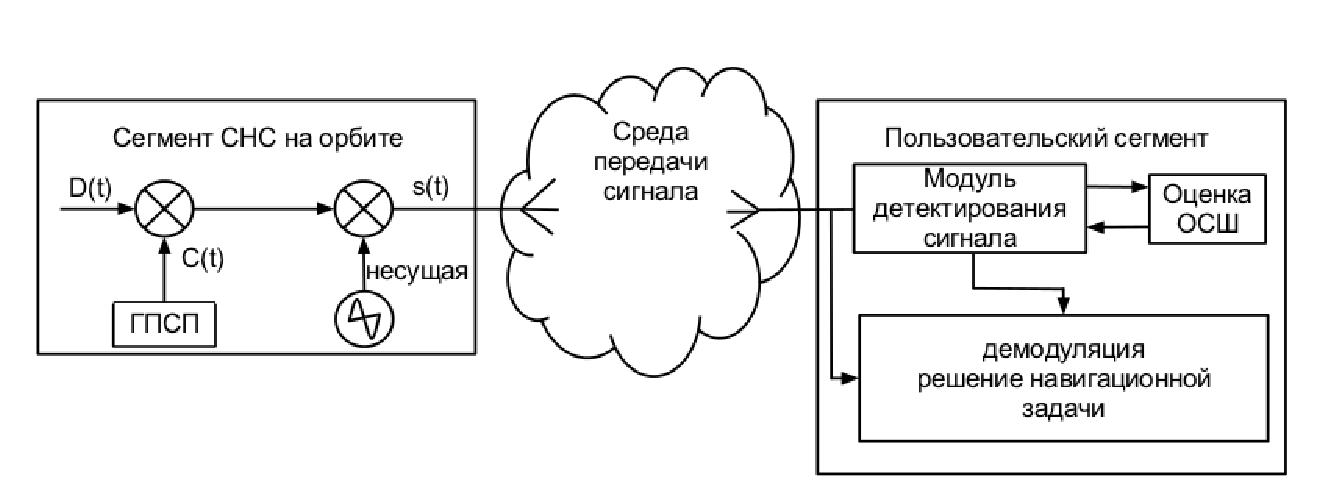
\includegraphics[width=1\linewidth]{sec1gnss_system.eps}}
\caption{структутраная схема СНС GPS}
\label{pic:sec1_gnss_system}
\end{figure}

В систему СНС GPS входят космический сегмент, наземный сегмент (на рисунке \ref{pic:sec1_gnss_system} не
отражен), а так же пользовательский сегмент. В космический сегмент входит спутниковая группировка, в 
наземный - станции управления, в пользовательский - все устройства принимающие сигнал от СНС GPS.

В данной работе рассматривается только пользовательский сегмент. В частности модули детектирования сигнала,
а так же модули оценки ОСШ принятого сигнала. Далее рассмотрены несколько алгоритмов детектирования сигнала,
а так же алгоритмов оценки ОСШ. Но до рассмотрения алгоритмов обработки сигнала, целесообразно кратко 
отразить свойства, а так же методы модулирования сигналов применяемых в СНС GPS.

\subsection{Свойства сигнала СНС GPS}
В системе СНС GPS применяются широкополосные сигналы (ШПС).
ШПС - сигналы, ширина полосы, используемой для передачи сигнала, которых
намного шире минимальной, необходимой для передачи данных \cite{sklyar}. Система связи считается системой с расширенным
спектром в следующих случаях \cite{sklyar}:

\begin{enumerate}
	\item Используемая полоса значительно шире минимальной, необходимой для передачи данных.
	\item Расширение спектра производится с помощью так называемого расширяющего (кодового) сигнала,
		который не зависит от передаваемой информации.
	\item Восстановление исходных данных ("сужение спектра") осуществляется путем сопостовления полученного
		сигнала и синхронизированной копии расширяющего сигнала
\end{enumerate}
Так же подобные сигналы называют:
\textquotedblleftсложными\textquotedblright,
\textquotedblleftшумоподобными\textquotedblright,
\textquotedblleftпсевдослучайными\textquotedblright,
\textquotedblleftсложными-дискретными\textquotedblright,
\textquotedblleftдискретно-кодированными\textquotedblright,
\textquotedblleftортогональными (квазиортогональными)\textquotedblright,
\textquotedblleftоптимальными дискретными\textquotedblright
\cite{gantmaher-book}.
Каждое название ставит акцент на определенной характеристике сигнала. В данной работе я буду оперировать термином
широкополосный сигнал - ШПС. ШПС можно определить как \cite{gantmaher-book, varakin-book}:

\begin{center}
\begin{equation}
	\label{eq:ss_signal}
	1 << FT = B,
\end{equation}
\end{center}
где: ${B}$ - база сигнала, ${F}$ - эффективная ширина спектра, а ${T}$ - длительность.
Неточность этого определеная рассмотрена в \cite{gantmaher-book}, так же там даны ссылки на другие источники
разделяющие критику данного определения. Для данной работы критика, рассмотренная в приведенных источниках,
принципального значения не имеет.

В данной работе используется сигнал с расширенным спектром методом "прямой последовательности". Данный метод
заключается в том, что несущая сигнала модулируется высокоскоростным (широкополосным) расширяющим сигналом \cite{sklyar}.
Методы генерации таких последовательностей рассмотрены, например, в \cite{gantmaher-book}. Это отдельная большая
тема для исследований. В данной работе используется ПСП - код Гоулда. Свойства ПСП подробно рассмотрены в
\cite{gold-ieee}, а так же краткое описание свойств без доказательства приведены в \cite{tsui, akos-book}.

Метод генерирования ПСП подробно рассмотрен во многих источниках \cite{tsui, akos-book, kaplan}
и в данной работе рассматриваться не будет.

В системе СНС GPS применяется двоичная фазовая манипуляция (ДФМ или в иностранной литературе BPSK).
В вышеприведенной системе несущее колебание ${\cos(\omega_{c}t})$ модулируется битами данных ${D_k(t)}$ и битами ПСП
${C_k{t}}$. Принимая во внимание, что потоки битов ${D_k(t)}$ и ${C_k{t}}$ могут принимать значения
${\{+1, -1\}}$. Определим входной сигнал как:

\begin{center}
\begin{equation}
	\label{eq:gps_signal}
	s_k(t) = \sqrt{2A}(C_k(t)D_k(t))\cos(\omega_{c}t)
\end{equation}
\end{center}
где: ${A}$ - мощность сигнала, ${C_k}$ - ПСП для ${k}$ - сигнала, ${D}$ - данные, а ${\omega_{c}t}$ - частота несущей сигнала.

Учитывая, что поток битов может принимать 2 дискретных значения, выражение \ref{eq:gps_signal} можно представить в виде \cite{sklyar}:
\begin{center}
\begin{equation}
	\label{eq:gps_signal_phase}
	s_k(t) = \sqrt{2A}\cos(\omega_{c}t + \phi_{i}(t))
\end{equation}
\end{center}
где: ${A}$ - мощность сигнала, ${\omega_{c}t}$ - частота несущей сигнала, а ${\phi_{i}(t)}$ - фаза несущей сигнала.

Поскольку мы имеем дело с ДФМ, фазовый член выражения \ref{eq:gps_signal_phase} может быть представлен как
${\phi_{i}(t) = \pi_{i}}$. На \ref{pic:sec1_bpsk} представлена несущяя сигнала с ДФМ.

\begin{figure}[ht]
\center\scalebox{0.7}{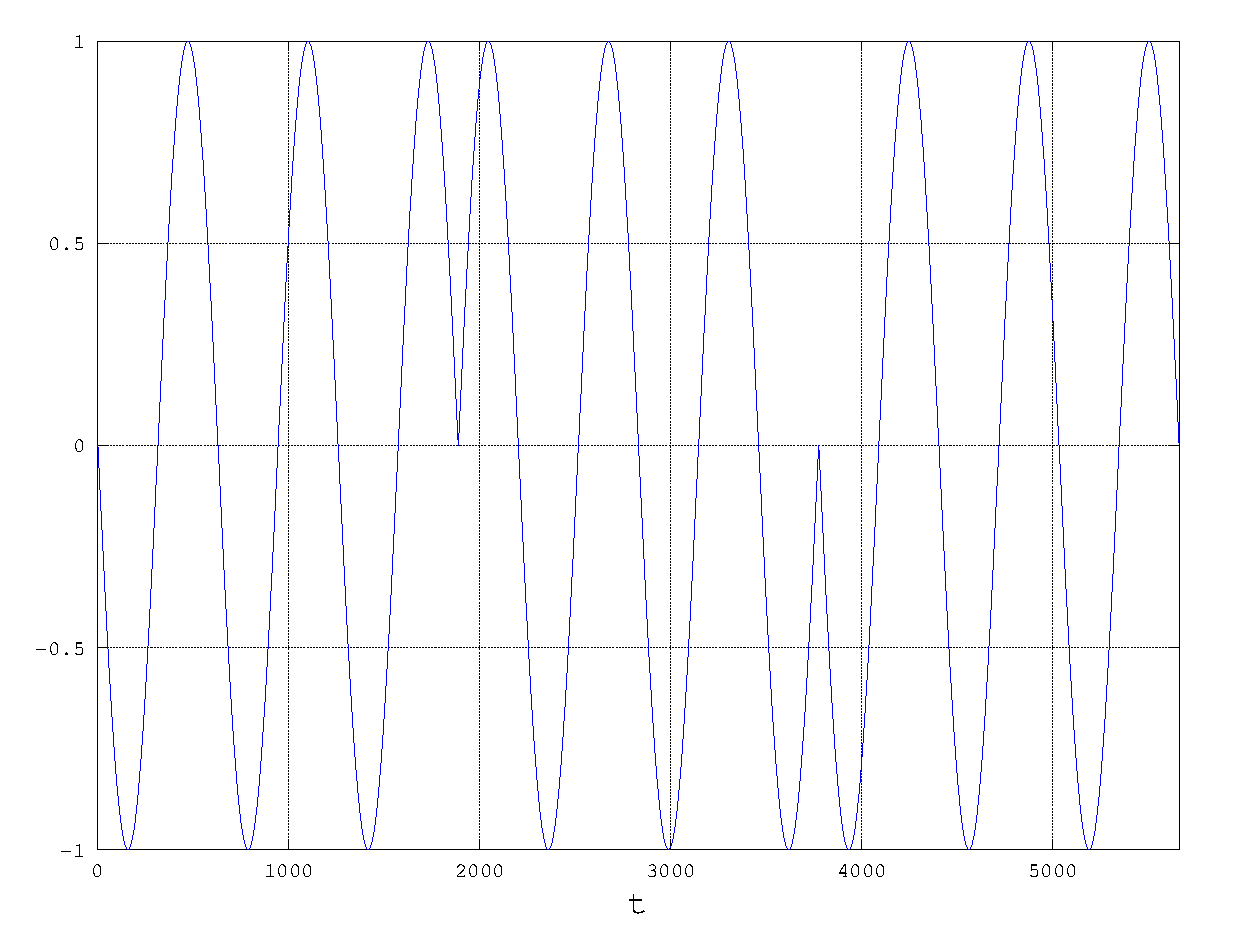
\includegraphics[width=1\linewidth]{bpsk.eps}}
\caption{Сигнал с модуляцией ДФМ}
\label{pic:sec1_bpsk}
\end{figure}
На рисунке \ref{pic:sec1_bpsk} представлена несущая, модулированная ДФМ.

Демодуляция производится повторной модуляцией принятого сигнала с синхронизированной копией ПСП ${C_k(t) - \tau}$, где
${\tau}$ - оценка фазы ПСП. При идеальной синхронизации сигнала, представленного вырежением \ref{eq:gps_signal},
c локальной копией ПСП, после демодуляции получаем:
\begin{center}
\begin{eqnarray}
	\label{eq:gps_signal_modulated}
	s_k(t) & = & \sqrt{2A}(C^2_k(t)D_k(t))\cos(\omega_{c}t) \\
	& = &\sqrt{2A}D_k(t)\cos(\omega_{c}t)
\end{eqnarray}
\end{center}
Таким образом, на выходе демодулятора получается сигнал с суженным спектром. Следует отметить, что правильная оценка ${\tau}$
является одной из основных задач при детектировании сигнала, так как ПСП имеет пик корреляции только в пределах центрального пика
АКФ \cite{gold-ieee}  - синхронизация с точностью до одного чипа. При неверной оценке фазы ПСП в результате демодуляции спектр
ШПС не будет сужен, что приведет к ошибочным результатам на следующих этапах решения: вычислении уровня шума и принятии решения
о наличии или отсутсивии сигнала заданного спутника в анализируемых данных.

\begin{figure}[H]
\center\scalebox{0.5}{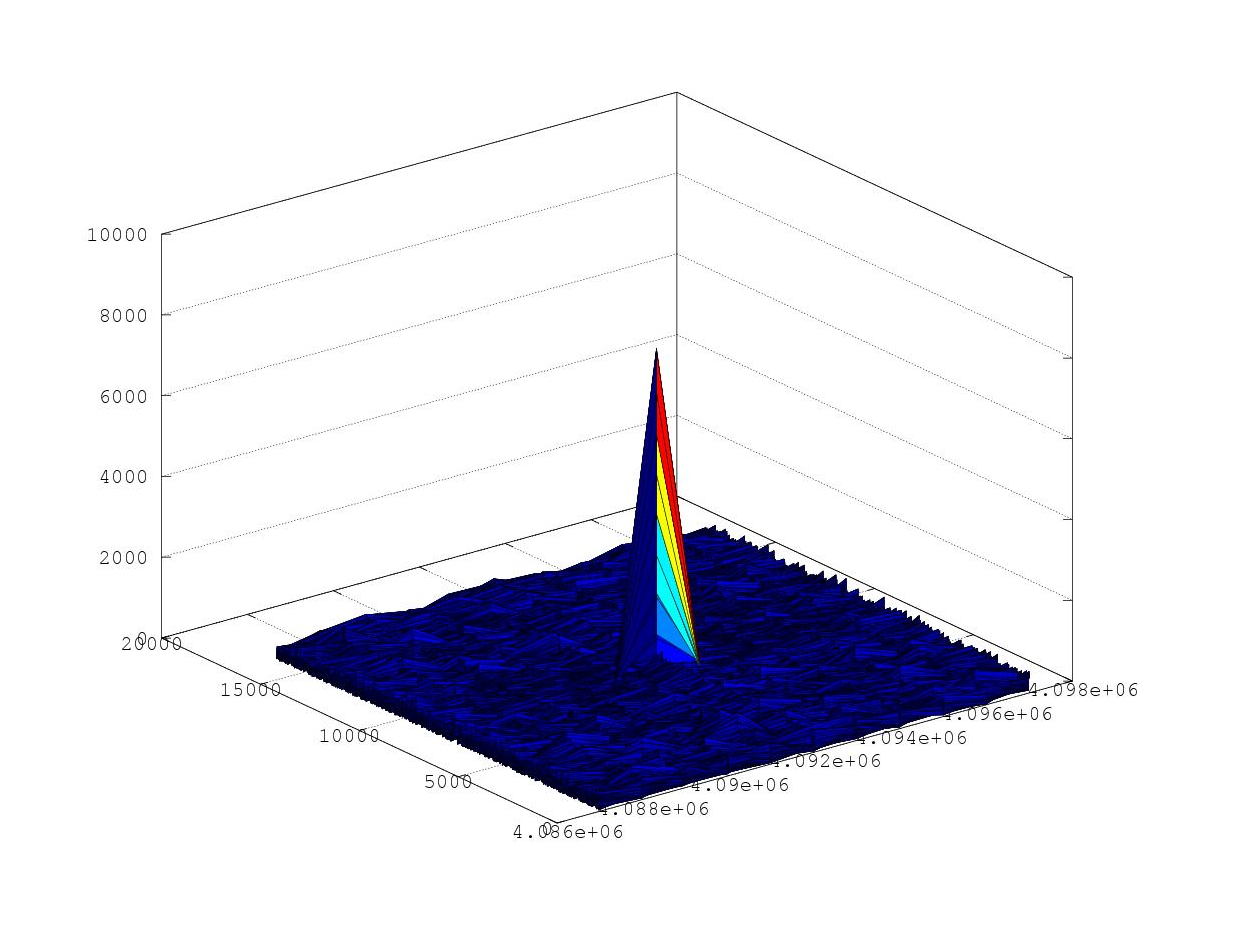
\includegraphics[width=1\linewidth]{corr_peak.eps}}
\caption{График ФН}
\label{pic:corr_peak}
\end{figure}

Задача поиска сигнала сводится к устранению неопределенности по двум параметрам: центральной частоте его спектра
и фазе ПСП. На рисунке \ref{pic:ambiguity_region} представлена область неопределенности. Можно заметить, что сечение
области неопределенности плоскостью ${f}$ представляет собой КФ сигнала. Поиск сигнала соответствует поиску и
оценке основного пика КФ.

\begin{figure}[H]
\center\scalebox{0.5}{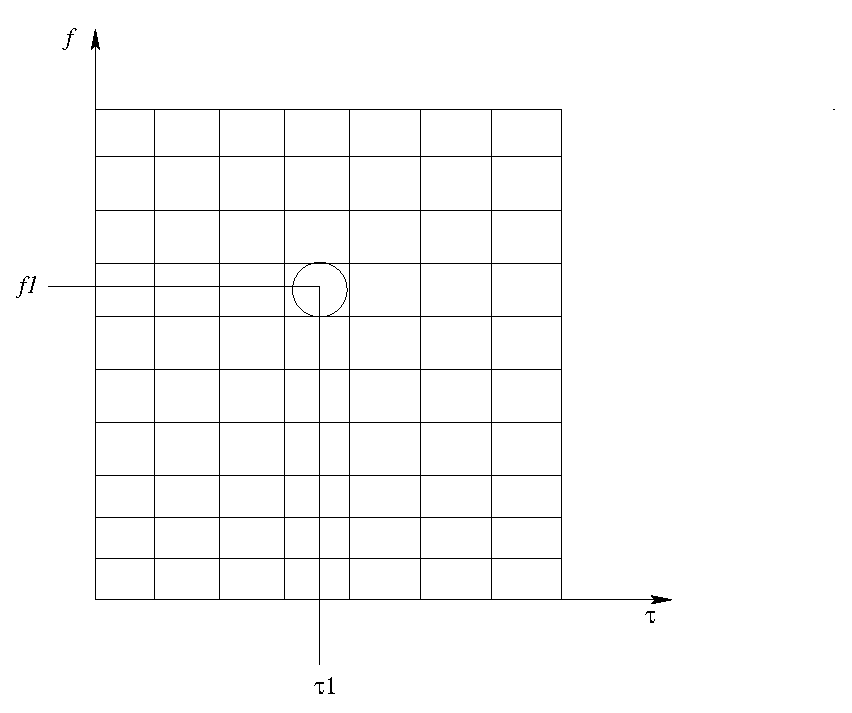
\includegraphics[width=1\linewidth]{ambiguity_region.eps}}
\caption{Область неопределенности}
\label{pic:ambiguity_region}
\end{figure}

\newpage
